
\documentclass[a4paper,12pt]{article}

% بسته‌های ریاضی برای معادلات و نمادهای پیشرفته
\usepackage{amsmath, amssymb, amstext, siunitx}

% بسته رنگ برای استفاده از رنگ در متن یا محیط‌ها
\usepackage{xcolor}

% بسته گرافیک برای درج تصاویر
\usepackage{graphicx}

% تنظیمات حاشیه صفحه
\usepackage{geometry}

% بسته لینک‌دهی (هایپرلینک‌ها)
\usepackage{hyperref}

% بسته صفحه‌آرایی برای تنظیم هدر و فوتر
\usepackage{fancyhdr}

% بسته xepersian برای پشتیبانی از زبان فارسی با XeLaTeX
\usepackage{xepersian}

% تعیین فونت فارسی (فایل فونت باید موجود باشد یا در سیستم نصب باشد)
\settextfont{B Nazanin}

% تنظیم اندازه حاشیه‌ها از هر طرف برابر با 1 اینچ
\geometry{margin=1in}

% تنظیم سبک fancy برای سربرگ و پاورقی
\pagestyle{fancy}

% سمت چپ هدر: مشخص‌کننده سری تمرین و نام درس
\lhead{تمرین سری سه درس فیزیک مدرن}

% وسط هدر: نام دانشکده
\chead{دانشکده فیزیک دانشگاه صنعتی خواجه نصیرالدین طوسی}

% سمت راست هدر: تاریخ روز به‌صورت خودکار
\rhead{\today}

% پایین صفحه: شماره صفحه
\cfoot{\thepage}

% شروع سند
\begin{document}
	
	% صفحه عنوان (بدون هدر و فوتر)
	\thispagestyle{empty}
	\begin{center}
		% لوگوی دانشگاه (در صورت وجود فایل تصویر در مسیر مشخص شده)
		
\includegraphics[width=0.5\textwidth]{../../../images/image-E_3/image-1.png} \\[10pt]
		% عنوان سند
		\textbf{\LARGE عنوان: تمرین سری سوم}\\[20pt]
		
		% نیم‌سال تحصیلی
		\textbf{\LARGE نیم‌سال تحصیلی: ۴۰۴۲ }\\[10pt]
		
		% نام مدرس درس
		\textbf{\Large مدرس: دکتر تقی‌زاده}\\[10pt]
		
		% مبحث تمرین
		\textbf{\Large مبحث تمرین: دینامیک نسبیتی }\\[10pt]
		
		% مهلت تحویل تمرین
		\textbf{\Large مهلت تحویل: ۲۲ خرداد}
	\end{center}
	
	% صفحه جدید برای ادامه سند
	\newpage
	
	% ایجاد فهرست مطالب به‌صورت خودکار (براساس \section ها)
	\tableofcontents
	\newpage
	
	\section{سوال اول}
	جعبه‌ای به ابعاد \( a, b, c \) به حال سکون در نظر بگیرید. جرم سکون آن \( m_0 \) و چگالی سکون آن \( \rho_0 = \frac{m_0}{abc} \) است.
	
	\begin{enumerate}
		\item حجم جعبه را از نظر ناظری به دست آورید که نسبت به آن با سرعت \( u \) در امتداد محور \( x \) حرکت می‌کند.
		\item جرم آن از نظر ناظر چه قدر است؟
		\item چگالی جعبه بر حسب \( \rho_0 \) از نظر ناظر چه قدر است؟
	\end{enumerate}
	
	\begin{center}
		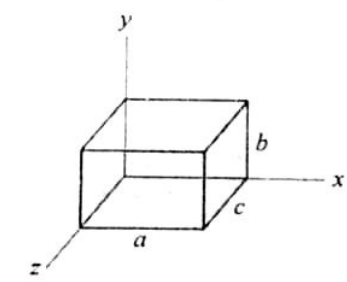
\includegraphics[width=0.5\textwidth]{../../../images/image-E_3/image-3.png}
	\end{center}
	
	\section{سوال دوم}
	قضیه کار-انرژی، تغییر انرژی جنبشی یک ذره را به کار انجام شده توسط نیروی خارجی روی آن مرتبط می‌سازد:
	
	\[\Delta K = W = \int F \, dx\]
	
	با نوشتن قانون دوم نیوتن به صورت \( F = dp/dt \)، نشان دهید:
	
	\[W = \int v \, dp\]
	
	و سپس با انتگرال‌گیری جزء به جزء و استفاده از تکانه‌ی نسبیتی، معادله \( K = (\gamma - 1)m_0 c^2 \) را به دست آورید.
	
	\section{سوال سوم}
	عمر متوسط مزون \( \mu \) (میون) در حال سکون \( 2/3 \times 10^{-4} \) ثانیه است. در یک اندازه‌گیری آزمایشگاهی عمر متوسط آن، \( 6/9 \times 10^{-4} \) ثانیه به دست می‌آید.
	
	\begin{enumerate}
		\item سرعت میون نسبت به اندازه‌گیری شده را محاسبه کنید.
		\item جرم سکون میون \( m_\mu = 207 m_e \) است. جرم موثر میون را وقتی به دست آورید که با این سرعت حرکت کند.
		\item انرژی جنبشی و تکانه‌ی آن چه قدر است؟
	\end{enumerate}
	
	\section{سوال چهارم}
	برای یک ذره به جرم \( m \)، در چه بازه‌ای از سرعت‌ها می‌توانیم از عبارت کلاسیک انرژی جنبشی \( \frac{1}{2}mv^2 \) با دقت ۱ درصد استفاده کنیم؟
	
	\section{سوال پنجم}
	کمیت \( c^2 t^2 - (x^2 + y^2 + z^2) \) مربوط به یک رویداد ناوردا (برای تمام ناظرها یکسان) و برابر \( c^2 \tau^2 \) است (\( \tau \) زمان ویژه).
	
	نشان دهید کمیت \( m_0^2 c^4 \) برای یک ذره ناوردا برابر \( E^2 - (p_x^2 + p_y^2 + p_z^2)c^2 \) است. یعنی:
	\[
	E^2 - p^2 c^2 = m_0^2 c^4
	\]
	
	\section{سوال ششم}
	اتم برانگیخته‌ای به جرم \( m \) در حالت اولیه‌ی ساکن در چارچوب \( S \) فوتونی گسیل می‌کند و پس می‌زند. کاهش انرژی داخلی اتم \( \Delta E \) و انرژی فوتون \( h\nu \) است. نشان دهید:
	
	\[ h\nu = \Delta E \left( 1 - \frac{\Delta E}{2mc^2} \right) \]
	
	\section{سوال هفتم}
	\begin{enumerate}
		\item نشان دهید بسامد زاویه‌ای بار متحرک در میدان مغناطیسی یکنواخت به صورت زیر است:
		\[ \omega = \frac{qB}{m} \sqrt{1 - \frac{u^2}{c^2}} \]
		\item این نتیجه را با نتیجه‌ی کلاسیکی که بعضی سیکلوتورون‌ها بر اساس آن طرح‌ریزی شده‌اند مقایسه کنید و به طور کیفی توضیح دهید از نظر نسبیتی. این طرح چگونه اصلاح شود؟
	\end{enumerate}
	
	\section{سوال هشتم}
	الکترونی با انرژی جنبشی 0.923 مگاالکترون‌ولت در حال حرکت است. سرعت آن چقدر است؟
	
	\section{سوال نهم}
	با توجه به شکل زیر رابطه:
	\[\frac{p^2}{2K} = m + \frac{K}{2c^2}\]
	را به دست آورید.
	
	\begin{center}
		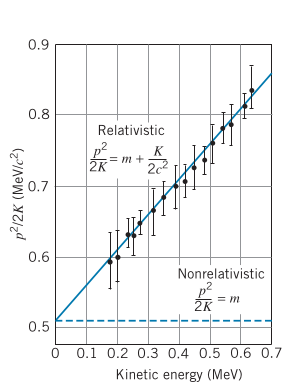
\includegraphics[width=0.5\textwidth]{../../../images/image-E_3/image-2.png}
	\end{center}
	
	\section{ سوال امتیازی اول}
	بار \( q \) در داخل میدان الکتریکی یکنواخت \( E \) در جهت مثبت محور \( x \) قرار دارد و در نقطه‌ی \( x = 0 \) از حال سکون، شتاب می‌گیرد.
	
	\begin{enumerate}
		\item نشان دهید شتاب بار از رابطه‌ی زیر به دست می‌آید:
		\[ a_x = \frac{qE}{m_0} \left( 1 - \frac{u^2}{c^2} \right)^{\frac{3}{2}} \]
		\item نشان دهید سرعت آن در زمان \( t \) از رابطه‌ی زیر به دست می‌آید:
		\[ u_x = \frac{qEt}{m_0 \sqrt{1 + \left( \frac{qEt}{m_0 c} \right)^2}} \]
		\item نشان دهید فاصله‌ی طی شده در مدت \( t \) از رابطه‌ی زیر به دست می‌آید:
		\[ x = \frac{m_0 c^2}{qE} \left[ \sqrt{1 + \left( \frac{qEt}{m_0 c} \right)^2} - 1 \right] \]
		\item نشان دهید برای مقادیر بزرگ \( t \)، \( u_x \) به سمت \( c \) میل می‌کند و \( x \) به صورت خطی با \( t \) افزایش می‌یابد.
		\item نشان دهید اگر \( \frac{qEt}{m_0} \ll c \) باشد، برای \( u_x \) و \( x \) نتایج کلاسیک به دست می‌آید.
	\end{enumerate}
	
	\section{سوال امتیازی دوم}
	ثابت کنید اگر \( \beta = \frac{u}{c} \ll 1 \) باشد، انرژی جنبشی ذره‌ی متحرک، \( K \)، همیشه خیلی کوچکتر از انرژی وابسته به جرم سکون آن \( m_0 c^2 \) خواهد بود.
	
	همچنین رابطه \( K = (m - m_0)c^2 \) را برای حرکت در فضای سه‌بعدی به دست آورید.
	
\end{document}